\chapter{Description}
\label{GameDescription}

The game begins with an NxN chess-like board where each square represents a potential position for the game
pieces. It contains grooves that runs between the squares where players can place their walls. Each player
is represented by a pawn represented by a character label that start on opposite sides, with their pawns
located at the center of their respective edge. The primary objective is to be the first player to move
their pawn to the row of squares on the opposite side of the game board avoiding any walls deterring its
path to the goal while strategically placing walls to deter opponents from reaching their goal squares.
\par
Walls are a fundamental element of the game, allowing players to strategically block their opponent's path
and influence the course of the game. Each wall spans across two cells and occupies exactly four cells either
horizontally or vertically, effectively creating a barrier between them. At the beginning, each player starts
with a set number of walls that they can use during their turn.

\begin{figure}[h]
    \centering
    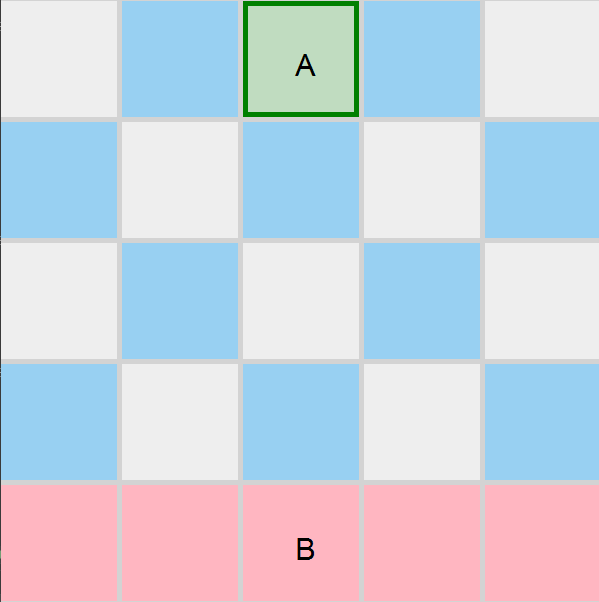
\includegraphics[scale=0.25]{../img/GameBoard/initial.png}
    \caption{A 5x5 game board}
    \label{fig:InitialGameBoard}
\end{figure}

As seen in figure \ref{fig:InitialGameBoard}, In the beginning, player A starts at cell (2, 0) and player B 
starts at cell (2, 4). A's goal is to reach the cells highlighted in pink. The gray areas between the cells
are grooves for wall placement.


\section{Notation}

There are no official notations for this game. However, some popular ones recognized by the Quoridor community
include \textbf{Glendenning's Notation} (\citep{Glendenning2002MasteringQ}) and the \textbf{Quoridor Strats Notation}
(\citep{website:COMMUNITY_NOTATION}). 
\par
Let $R = \{a, ..., i\}$ and $C = \{1, ..., 9\}$
\newline
Both notations follow the same principle of labelling each cell by $C_{ij}$ where $i \in R$ and $j \in C$.
\newline
Move $M$ and Wall $W$ are denoted algebraically, where
\par
$M(C_{ij}) = ij$ where $i \in R$ and $j \in C $,
\par
$W(C_{ij}) = ijD$ where $i \in R$, $j \in C$ and $D \in \{h, v\}$
\newline
\newline
The difference between the two notations is the way the walls are represented.

\begin{figure}[h]
    \begin{subfigure}{0.4\textwidth}
      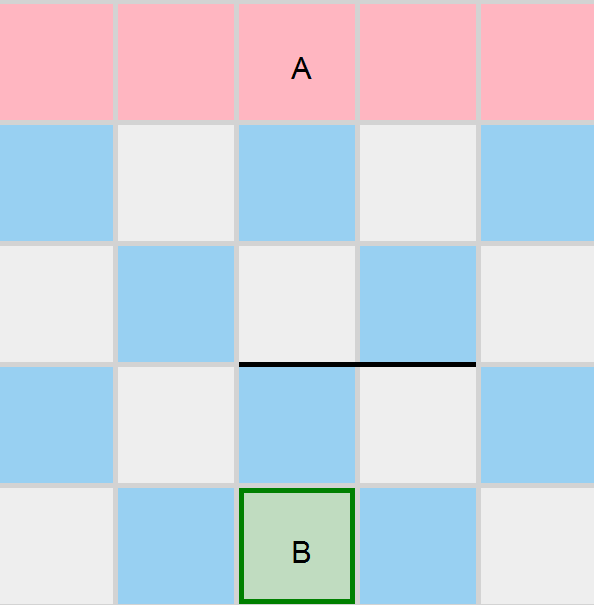
\includegraphics[width=\textwidth]{../img/GameBoard/wall_repr.png}
      \caption{Glendenning's Notation: \textbf{c3h}}
      \label{fig:NotationDifferentA}
    \end{subfigure}
    \hfill
    \begin{subfigure}{0.4\textwidth}
      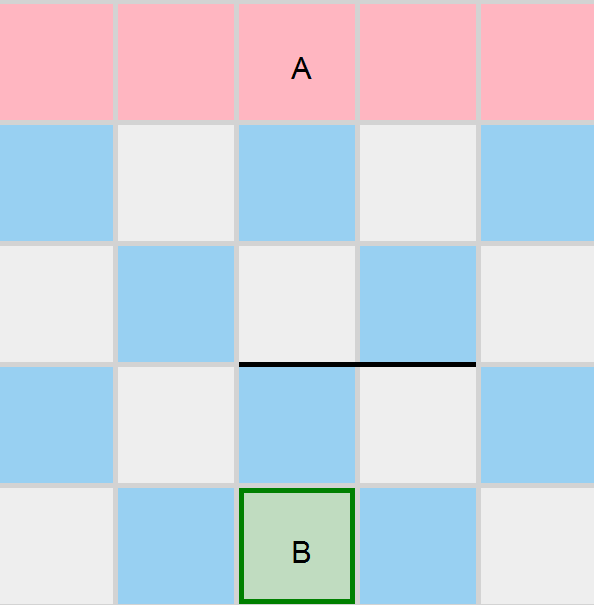
\includegraphics[width=\textwidth]{../img/GameBoard/wall_repr.png}
      \caption{Quoridor Strats Notation: \textbf{c4h}}
    \end{subfigure}
    \caption{Notation differences}
    \label{fig:WallNotationsDifferent}
\end{figure}

As seen in Figure \ref{fig:WallNotationsDifferent}, the difference lies in the point of reference of the wall.
In \textbf{Quoridor Strats Notation}, each wall coordinate is represented by the lower-left cell the wall
follows along, whereas in \textbf{Glendenning's Notation}, each wall is represented by the upper-left cell the
wall follows along.


Even though they are widely used, they are very easy to get confused with since they have the same wall representations,
and unless specified explicitly, it is difficult to tell which representation is being used.
\par
This is why I have decided to use a different representation for walls. Instead of vertical and horizontal wall
with respect to a cell, we define a direction explicitly.
\par
$W(C_{ij}) = ijD$ where $i \in R$, $j \in C$ and $D \in \{N, S, E, W\}$
\newline
Looking back at Figure \ref{fig:NotationDifferentA}, the walls can now be represented by \textbf{c4N}, i.e. a
Northern wall from the cell $C_{c4}$.

\pagebreak

\section {Rules}

\subsection{Wall placement rules}
\label{WallRules}

\begin{itemize}
    \item Walls cannot be placed diagonally.
    \item A placed wall must not completely block any player's path to victory. Each player must have at least
        one path to victory \textit{(See figure \ref{fig:WallBlockingMove})}
    \item A placed wall cannot intersect any of the previously placed walls.
    \item Walls cannot be placed along the edges of the board. Walls must be placed to create a barrier for
        exactly 4 cells
    \item  Every player possesses a limited supply of walls, and once they exhaust these walls, they are unable
        to place any additional ones. Consequently, the player is only allowed to maneuver their pawn on the
        board.
\end{itemize}

\begin{figure}[h]
    \begin{subfigure}{0.4\textwidth}
      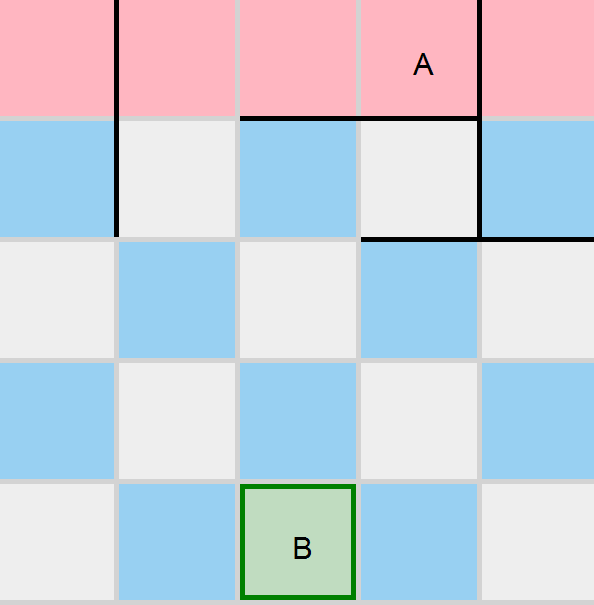
\includegraphics[width=\textwidth]{../img/GameBoard/arbitrary_state.png}
      \caption{Valid game state}
      \label{fig:ValidState}
    \end{subfigure}
    \hfill
    \begin{subfigure}{0.4\textwidth}
      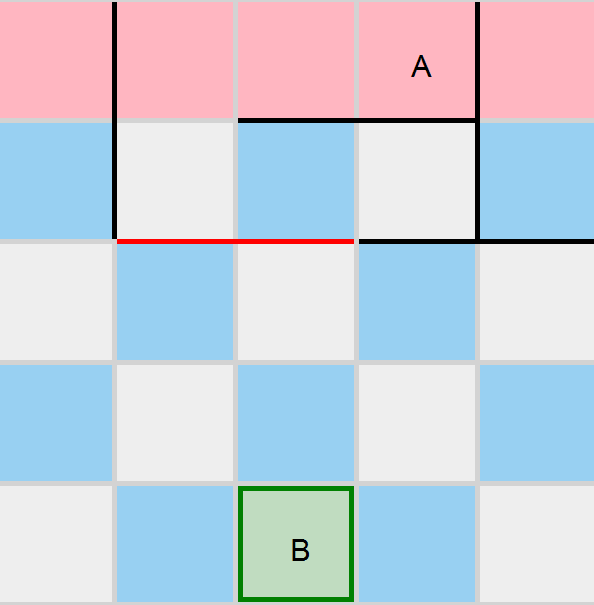
\includegraphics[width=\textwidth]{../img/GameBoard/invalid_wall.png}
      \caption{Invalid game state}
      \label{fig:WallBlocked}
    \end{subfigure}
    \caption{Example of an invalid wall placement}
    \label{fig:WallBlockingMove}
\end{figure}

The game state represented by Figure \ref{fig:ValidState} shows the situation after 5 turns, with it currently
being player B's turn to move. Since both \textbf{A} and \textbf{B} have viable paths to their respective goal
rows and all walls have been placed according to the rules (see \textit{Section \ref{WallRules}}),
the game state shown in Figure \ref{fig:ValidState} is considered valid.
\par
However, player B disrupts the rules by placing the red wall, violating the specified wall-placement rules
(see \textit{Section \ref{WallRules}}), consequently rendering the game state represented by
Figure \ref{fig:WallBlocked} invalid.

\pagebreak

\subsection{Player movement rules}

\begin{itemize}
    \item Players are allowed to move their pawn one unit at a time in the North, South, East, or West
        directions during their turn. Diagonal movements are not allowed.

    \item \textbf{Jump}
    \begin{itemize}
        \item If an opponent is at to the cell a player intends to move to, the player can jump over the
            opponent provided there is no wall between them or behind the opponent they intend to jump over.
            In the latter case, the player can jump to a cell on either side of the opponent's cell, given
            the cell is accessible from the opponent's cell.
        \item Players cannot jump over walls
        \item A Player is allowed to jump over multiple opponents as long as they adhere to the aforementioned
            conditions.
    \end{itemize}
\end{itemize}

\begin{figure}[h]
    \begin{subfigure}{0.2\textwidth}
      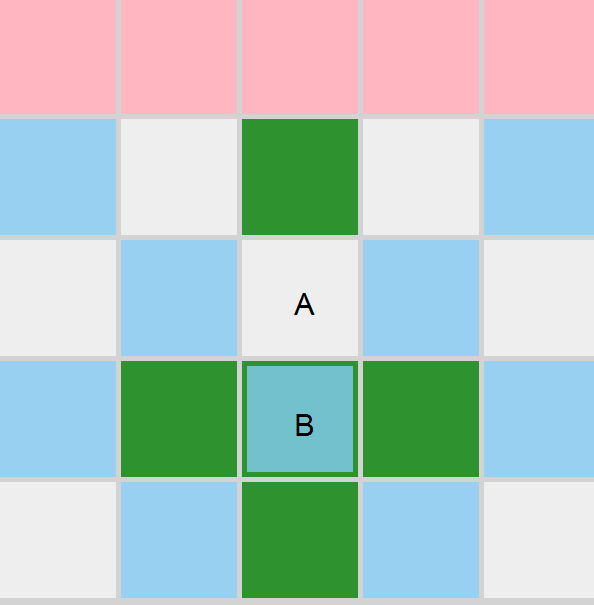
\includegraphics[width=\textwidth]{../img/GameBoard/move01.png}
    \end{subfigure}
    \hfill
    \begin{subfigure}{0.2\textwidth}
        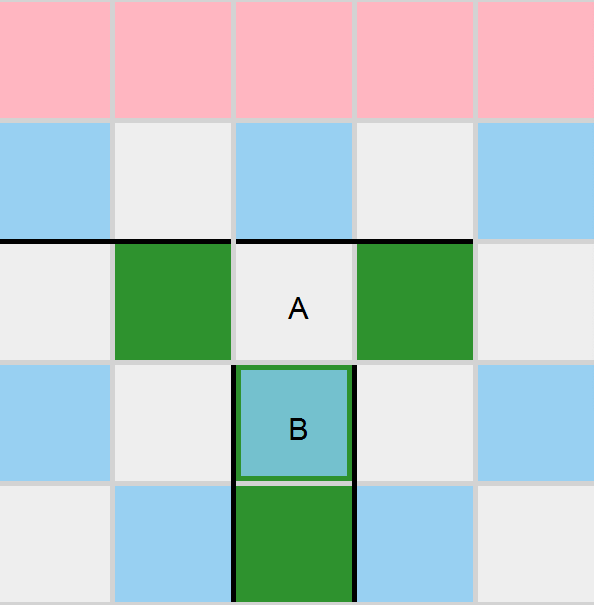
\includegraphics[width=\textwidth]{../img/GameBoard/move02.png}
    \end{subfigure}
    \hfill
    \begin{subfigure}{0.2\textwidth}
        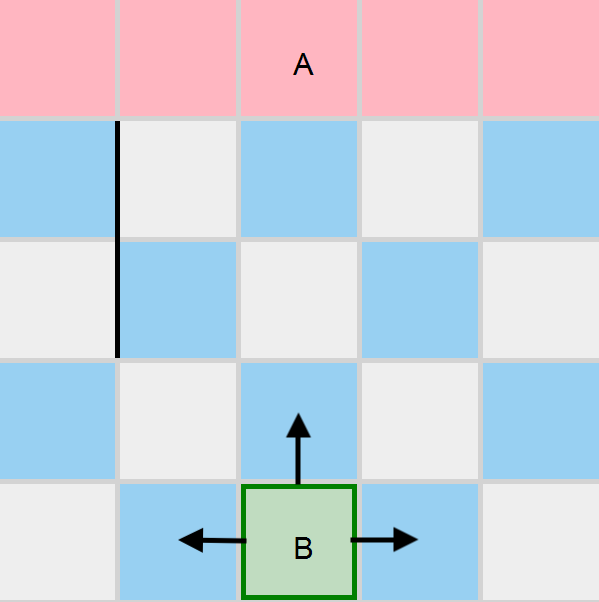
\includegraphics[width=\textwidth]{../img/GameBoard/move03.png}
    \end{subfigure}
    \hfill
    \begin{subfigure}{0.2\textwidth}
        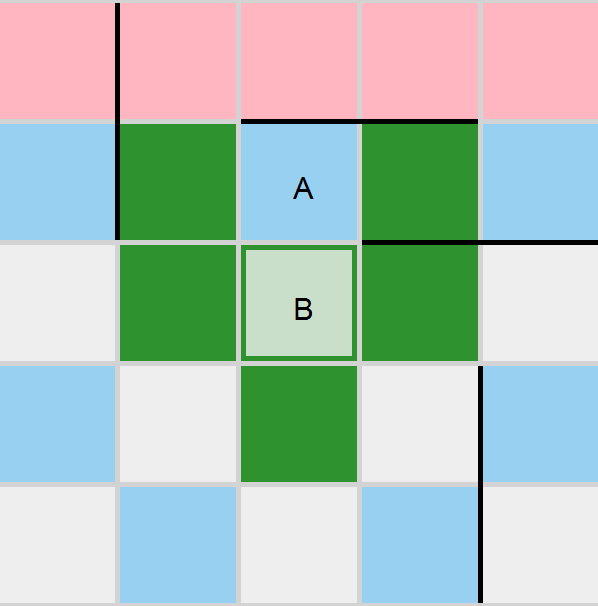
\includegraphics[width=\textwidth]{../img/GameBoard/move04.png}
    \end{subfigure}
    \caption{Examples of possible moves for player B in the game state}
    \label{fig:PossibleMoves}
\end{figure}